\notechapter{N-20250118}{Schemes Gently: Prime Ideals as Points and Functions as Local Data}

\section{Why schemes appear}

Affine varieties are built from polynomial equations over algebraically closed fields. Schemes enlarge this world. They allow arithmetic examples, nilpotents, and spaces that are glued from affine pieces.

The first definition is surprisingly short:
\[
  \operatorname{Spec}R=\{\mathfrak p\subset R:\mathfrak p\text{ is a prime ideal}\}.
\]
A scheme begins by treating prime ideals as points.

\section{Prime ideals as generalized points}

For \(R=k[x]\), maximal ideals \((x-a)\) correspond to ordinary points \(a\in k\). But \((0)\) is also a prime ideal. It is a generic point: it is not one location, but the whole irreducible line viewed algebraically.

Thus \(\operatorname{Spec}R\) contains more than classical points. It contains information about irreducible pieces and specialization.

\section{Closed sets and opens}

For an ideal \(I\subset R\), define
\[
  V(I)=\{\mathfrak p\in\operatorname{Spec}R:I\subseteq\mathfrak p\}.
\]
These sets are closed in the Zariski topology.

The distinguished open set associated to \(f\in R\) is
\[
  D(f)=\{\mathfrak p:f\notin\mathfrak p\}.
\]
One should read \(D(f)\) as the region where \(f\) is allowed to be inverted.

\section{Examples}

For a field \(k\), \(\operatorname{Spec}k\) has one point.

For \(k[x]\), \(\operatorname{Spec}k[x]\) contains closed points \((x-a)\) and the generic point \((0)\).

For \(\mathbb Z\), \(\operatorname{Spec}\mathbb Z\) has points \((p)\) for each prime number \(p\), together with the generic point \((0)\). This is why people say \(\operatorname{Spec}\mathbb Z\) behaves like an arithmetic curve.

\section{Nilpotents and the double point}

Consider
\[
  R=k[x]/(x^2).
\]
The element \(x\) is nonzero but nilpotent:
\[
  x^2=0.
\]
The topological space \(\operatorname{Spec}R\) has only one point, but the ring remembers an infinitesimal thickening at that point.

This is one of the main reasons schemes are useful. They do not throw away nilpotent information.

\section{The structure sheaf}

A space is not enough. We also need functions on it. On a distinguished open \(D(f)\), the functions are given by localization:
\[
  \mathcal O_{\operatorname{Spec}R}(D(f))=R_f.
\]
Here \(R_f\) means that powers of \(f\) are allowed in denominators.

This formula is the computational heart of affine schemes.

\section{Stalks and local rings}

At a prime ideal \(\mathfrak p\), the stalk of the structure sheaf is
\[
  \mathcal O_{\operatorname{Spec}R,\mathfrak p}=R_{\mathfrak p}.
\]
This is a local ring. It focuses on functions near the point \(\mathfrak p\) by inverting elements not in \(\mathfrak p\).

The local ring is the algebraic version of a small neighborhood.

\section{A safe mental model}

A scheme is not just a set of prime ideals. It is a space with a sheaf of rings. The points tell us where we are; the rings tell us what functions are available near each point.

\[
\begin{array}{c|c}
\text{scheme idea} & \text{meaning}\\
\hline
\operatorname{Spec}R & \text{prime ideals as points}\\
V(I) & \text{closed condition}\\
D(f) & \text{place where }f\text{ is invertible}\\
R_f & \text{functions on }D(f)\\
R_{\mathfrak p} & \text{functions near }\mathfrak p
\end{array}
\]

%% expanded-on-review

\section{The topology of the affine line spectrum}

The space \(\operatorname{Spec}k[x]\) has a generic point \((0)\) and closed points \((x-a)\). The closure of the generic point is the whole space:
\[
  \overline{\{(0)\}}=\operatorname{Spec}k[x].
\]
The closure of \((x-a)\) is just itself.

This is very different from ordinary Hausdorff geometry. But it is meaningful: the generic point represents the whole irreducible line, while a closed point represents a particular value of \(x\).

\begin{center}
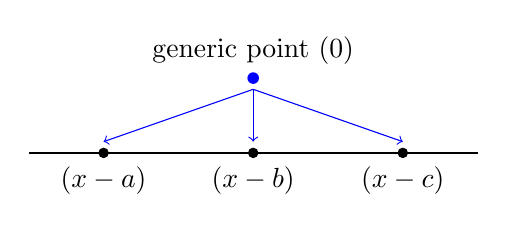
\begin{tikzpicture}[scale=0.95]
  \draw[thick] (-3,0) -- (3,0);
  \foreach \x/\lab in {-2/{(x-a)},0/{(x-b)},2/{(x-c)}} {
    \fill (\x,0) circle (2pt);
    \node[below] at (\x,-.05) {$\lab$};
  }
  \fill[blue] (0,1.0) circle (2.2pt);
  \node[above] at (0,1.05) {generic point $(0)$};
  \draw[->,blue] (0,.85) -- (-2,.15);
  \draw[->,blue] (0,.85) -- (0,.15);
  \draw[->,blue] (0,.85) -- (2,.15);
\end{tikzpicture}
\end{center}

The arrows are only suggestive: the generic point specializes to closed points.

\section{Localization as zooming in}

For a prime ideal \(\mathfrak p\), the local ring
\[
  R_{\mathfrak p}
\]
is obtained by inverting everything not in \(\mathfrak p\). This means that near \(\mathfrak p\), functions not vanishing there are treated as units.

For \(R=k[x]\) and \(\mathfrak p=(x-a)\), the local ring
\[
  k[x]_{(x-a)}
\]
contains rational functions whose denominators do not vanish at \(a\). This is exactly the algebraic version of functions defined near \(a\).

\section{Why nilpotents are geometric}

The ring \(k[x]/(x^2)\) has the same classical point as \(k[x]/(x)\), but it has more infinitesimal information. The element \(x\) is not zero, yet its square is zero.

A useful mental picture is that \(\operatorname{Spec}k[x]/(x^2)\) is a point with a first-order tangent fuzz. The point cannot be separated into two visible points, but algebra can still detect a direction of infinitesimal thickening.



\section{Why the spectrum of the integers is geometric}

The points \((p)\) of \(\operatorname{Spec}\mathbb Z\) behave like closed points, one for each prime number. The point \((0)\) behaves like a generic point. An integer \(n\) vanishes at exactly the prime ideals \((p)\) with \(p\mid n\).

Thus divisibility becomes geometry:
\[
  V(n)=\{(p):p\mid n\}.
\]
This is one of the most charming reasons schemes are worth learning: arithmetic starts to look like a geometric space.


\section{What to remember}

Schemes are a controlled generalization of algebraic varieties. They keep ordinary points, generic points, arithmetic points, and infinitesimal information in one language.

The main idea is not to make geometry obscure. It is to let algebraic geometry keep the information that classical point sets forget.
